\documentclass{standalone}
\usepackage{amsmath}
\usepackage{tikz}
\begin{document}
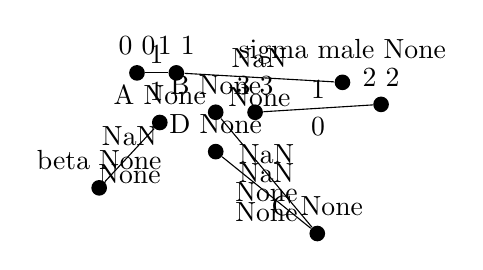
\begin{tikzpicture}
\node[fill=black, circle, inner sep=2pt, label=above:{\textcolor{black}{$\text{0}$} \textcolor{black}{0}}] (Graph with 5 nodes and 3 edgesN0) at (3.7,-0.2) {};
\node[fill=black, circle, inner sep=2pt, label=above:{\textcolor{black}{$\text{1}$} \textcolor{black}{1}}] (Graph with 5 nodes and 3 edgesN1) at (4.2,-0.2) {};
\node[fill=black, circle, inner sep=2pt, label=above:{\textcolor{black}{$\text{sigma male}$} \textcolor{black}{None}}] (Graph with 5 nodes and 3 edgesNsigma male) at (6.31,-0.32) {};
\node[fill=black, circle, inner sep=2pt, label=above:{\textcolor{black}{$\text{2}$} \textcolor{black}{2}}] (Graph with 5 nodes and 3 edgesN2) at (6.8,-0.6) {};
\node[fill=black, circle, inner sep=2pt, label=above:{\textcolor{black}{$\text{3}$} \textcolor{black}{3}}] (Graph with 5 nodes and 3 edgesN3) at (5.2,-0.7) {};
\draw[draw=black, shorten >=3pt, shorten <=3pt] (3.7,-0.2) -- (4.2,-0.2);
\node[above, text=black] at (3.95,-0.2) {\textcolor{black}{1}};
\node[below, text=black] at (3.95,-0.2) {\textcolor{black}{1}};
\draw[draw=black, shorten >=3pt, shorten <=3pt] (4.2,-0.2) -- (6.31,-0.32);
\node[above, text=black] at (5.255,-0.26) {\textcolor{black}{NaN}};
\node[below, text=black] at (5.255,-0.26) {\textcolor{black}{None}};
\draw[draw=black, shorten >=3pt, shorten <=3pt] (6.8,-0.6) -- (5.2,-0.7);
\node[above, text=black] at (6.0,-0.65) {\textcolor{black}{1}};
\node[below, text=black] at (6.0,-0.65) {\textcolor{black}{0}};
\node[fill=black, circle, inner sep=2pt, label=above:{\textcolor{black}{$\text{A}$} \textcolor{black}{None}}] (Graph with 5 nodes and 3 edgesNA) at (3.99,-0.83) {};
\node[fill=black, circle, inner sep=2pt, label=above:{\textcolor{black}{$\text{beta}$} \textcolor{black}{None}}] (Graph with 5 nodes and 3 edgesNbeta) at (3.22,-1.66) {};
\node[fill=black, circle, inner sep=2pt, label=above:{\textcolor{black}{$\text{C}$} \textcolor{black}{None}}] (Graph with 5 nodes and 3 edgesNC) at (5.99,-2.24) {};
\node[fill=black, circle, inner sep=2pt, label=above:{\textcolor{black}{$\text{B}$} \textcolor{black}{None}}] (Graph with 5 nodes and 3 edgesNB) at (4.7,-0.7) {};
\node[fill=black, circle, inner sep=2pt, label=above:{\textcolor{black}{$\text{D}$} \textcolor{black}{None}}] (Graph with 5 nodes and 3 edgesND) at (4.7,-1.2) {};
\draw[draw=black, shorten >=3pt, shorten <=3pt] (3.99,-0.83) -- (3.22,-1.66);
\node[above, text=black] at (3.605,-1.245) {\textcolor{black}{NaN}};
\node[below, text=black] at (3.605,-1.245) {\textcolor{black}{None}};
\draw[draw=black, shorten >=3pt, shorten <=3pt] (4.7,-0.7) -- (5.99,-2.24);
\node[above, text=black] at (5.345,-1.47) {\textcolor{black}{NaN}};
\node[below, text=black] at (5.345,-1.47) {\textcolor{black}{None}};
\draw[draw=black, shorten >=3pt, shorten <=3pt] (5.99,-2.24) -- (4.7,-1.2);
\node[above, text=black] at (5.345,-1.72) {\textcolor{black}{NaN}};
\node[below, text=black] at (5.345,-1.72) {\textcolor{black}{None}};
\end{tikzpicture}
\end{document}
